The first part of our all-atom fitting algorithm is to fit the protein backbone to the given \Ca-trace ignoring side-chain conformations.

As input we are given a \Ca-trace target and a protein in form of an amino acid sequence.
Only the amino acid types are provided; no spatial structure information about the protein is given as this is left to the fitting algorithm to find.


\section{Limitations}
The adjustable parameters in a protein backbone structure consists of bond angles, dihedral angles and bond lengths.
As the dihedral angles are by far the most influential parameters we allow ourselves to perform the simplification of not considering bond lengths and bond angles.
More specifically, we will only adjust the $\phi$ and $\psi$ angles on the atom bonds between \Ca-C and \Ca-N.
For all other parameters we use known constants that approximate the average backbone structure.
Thus, the protein backbone to be folded becomes a sequence of identical amino acid backbones that can only be modified by adjusting $\phi$ and $\psi$ for each amino acid.


\section{Inverse kinematics}
With the above limitations in place the backbone fitting problem can be regarded as an \emph{inverse kinematics} (IK) problem.
IK is the process of determining angles of joints in a chain of rigid links in order to make the end of the linked chain reach a desired position in space.
The end of the the linked chain is called the \emph{end-effector}.

In our case, the spatial structure consists of a series of atoms (joints) connected by atom bonds (links).
Our backbone fitting problem is not an ordinary IK problem since we have multiple end-effectors in form of the target \Ca-trace.

To simplify the problem, we can separately consider each backbone \Ca\ as an end-effector that must reach its corresponding target \Ca.
In this way the problem is decomposed into many small IK problems.
However, this simplification is not entirely valid as the entire backbone cannot be fitted by solving many local problems.
For example, a configuration of $\phi$ and $\psi$ angles might fit a single \Ca\ well to its target, but in such a way that the next \Ca\ in the backbone cannot come close to its target.
Therefore, a good solution should take global context into account when solving IK problems locally. 

%An IK problem may have multiple solutions depending on the number of degrees of freedom (DOF) given by the adjustable angles.
%In our fitting problem, we just want a single solution.
%In most cases, however, there is no solution as our limitations make it impossible to conform to a given \Ca-trace.
%Furthermore, it is possible that the given \Ca-traces have a completely unrealistic structure.
%In these cases, we just want a solution that is somewhat close to the target.

%As we have decided not to consider the bond angles (joint angles), the only adjustable angles in the kinematic chain are the dihedral angles around the atom bonds between \Ca-C and \Ca-N.


\section{Related work}
Several IK solving methods exist and have been utilized in protein
structure prediction.  However, these methods are mainly concerning
the \emph{loop closure} problem \cite{coutsias2004kinematic} which
differs from our problem since the only constraint is that the
positions of both chain ends must be locked. In these problems the
chains are also often relatively small (typically 4-14 amino acids),

  
Shenkin et al. describe a Jacobian solution in which the partial derivatives model the movement of the end of the kinematic chain relative to the angular changes, \cite{shenkin1987}.
To calculate the necessary angular changes the Jacobian is simply inverted.
The method then works iteratively by calculating the angular changes and adjusting the angles correspondingly in each step in order to move the end effector towards its target.
%Moreover, the method is capable of handling lower limit constraints on interatomic distances between the end.

The Jacobian approach has one downside according to Canutescu and Dunbrack
\cite{canutescu2003}.
If the Jacobian matrix is close to singular by coincidence, the inversion is ill posed yielding unstable results.
Instead, they propose a \emph{cyclic coordinate descent} (CCD) method.
CCD decomposes the problem by solving one angle at a time wrt. the end-effector.
1 DOF problems are simple and can be solved analytically.
This is done repeatedly up the link chain, making the end-effector position converge towards the target.
To give more realistic results, a Ramachandran probability map is used to determine if a proposed angle is acceptable. 
It is claimed that their method has very fast performance. 
However, the algorithm may fail to find solutions for short amino acid sequences.
In \cite{boomsma2005full}, the CCD method is extended to include bond angles.

Finally, Wedemeyer and Scheraga has proposed a method for solving loop closures with 3 amino acides (6 DOFs) in closed form by reducing the problem to extracting roots of a polynomial, \cite{wedemeyer1999exact}.


\section{Cyclic coordinate descent}
For the backbone fitting problem we have chosen to experiment with the CCD approach as it is simple, fast, numerically stable and flexible (ie. it is easy to introduce algorithmic constraints).

In this section, we present a single step in the CCD method.
Figure \ref{fig:ccd} illustrates the situation.
CCD works iteratively by adjusting one angle at time according to the end-effector.
In this case the angle to be adjusted is the $\phi$ angle around the bond between N and C$_{\alpha0}$. Moreover, the end-effector consist of three consecutive backbone \Ca-atoms after C$_{\alpha0}$.

\begin{figure}
  \centering
	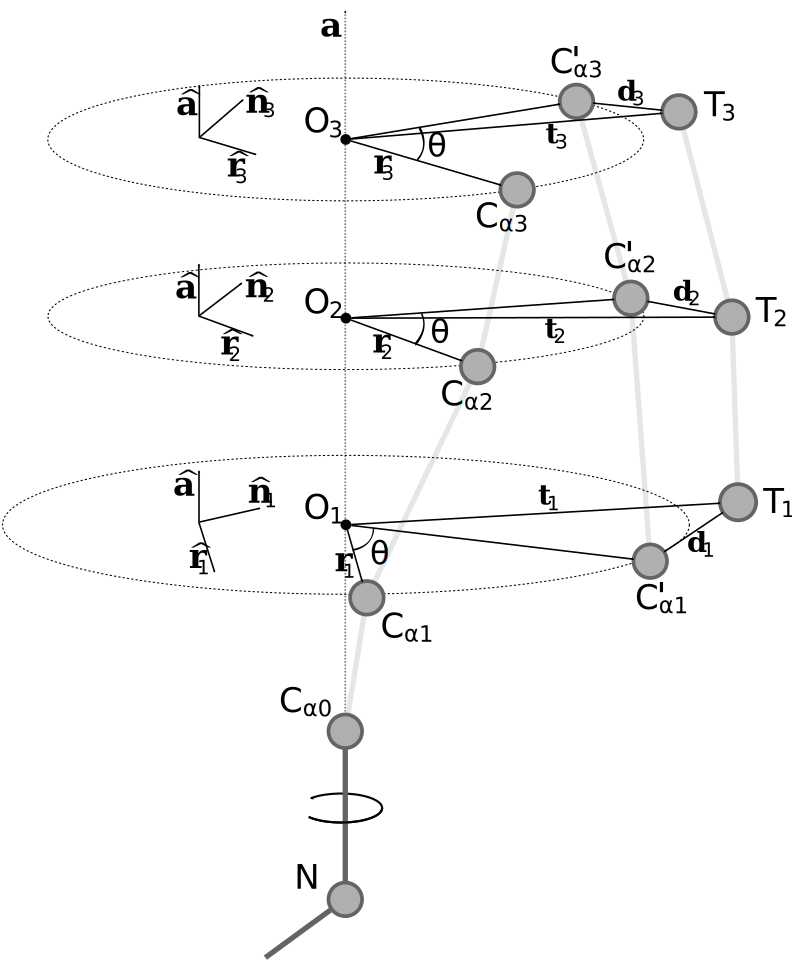
\includegraphics[width=0.98\columnwidth]{figures/ccd}
  \caption{Adjusting an angle with the CCD algorithm.}
  \label{fig:ccd}
\end{figure}


In the illustration, T$_{1-3}$ denote the end-effector target (from the \Ca-trace). O$_{1-3}$ are the projections of C$_{\alpha1-3}$ on the rotation axis. C$_{\alpha1-3}$ and C$'_{\alpha1-3}$ denote the position of the end-effector before and after the rotation respectively.
For $i=1,2,3$ we denote the vectors
 $$\v{r}_i = \overrightarrow{\text{O}_i\text{C}}_{\alpha i}~~,~~ \v{t}_i = \overrightarrow{\text{O}_i\text{T}}_{\alpha i} , $$
$$\v{d}_i = \overrightarrow{\text{T}_i\text{C}}'_{\alpha i} = \overrightarrow{\text{O}_i\text{C}}'_{\alpha i}-\overrightarrow{\text{O}_i\text{T}}_{\alpha i}$$

To compute $\overrightarrow{\text{O}_i\text{C}}'_{\alpha i}$, we define a local coordinate system from the orthogonal vectors $\hat{\v{r}}_i, \hat{\v{a}}, \hat{\v{n}}_i$ with $\hat{\v{r}}_i$ being the unit vector of $\v{r}_i$, $\hat{\v{a}}$ being the unit vector of the rotation axis $\v{a}$ and $\v{n}_i = \hat{\v{a}} \times \hat{\v{r}}_i$. We can now compute the vector by:
$$\overrightarrow{\text{O}_i\text{C}}'_{\alpha i} = \hat{\v{r}}_i||\v{r}_i||\cos\theta + \hat{\v{n}}_i||\v{r}_i||\cos\theta$$
And thus, $\v{d}_i$ is given by
$$\v{d}_i =  \hat{\v{r}}_i||\v{r}_i||\cos\theta + \hat{\v{n}}_i||\v{r}_i||\cos\theta - \v{t}_i$$

The rotation $\theta$ around $\v{a}$ is chosen such that the sum of square distances $S$ between the rotated end-effectors and their targets are minimized.
$$S=||\v{d}_1||^2+||\v{d}_2||^2+||\v{d}_3||^2$$
with the square distance of $\v{d}_i$ given by
\begin{eqnarray*}
||\v{d}_i||^2 &=& ||\v{r}_i||^2 + ||\v{t}_i||^2 - 2(\v{t}_i\cdot\hat{\v{r}}_i)||\v{r}_i||\cos\theta\\
&& - 2(\v{t}_i\cdot\hat{\v{n}}_i)||\v{r}_i||\sin\theta
\end{eqnarray*}

To find the extreme values of $S$ we take the first-order derivative wrt. $\theta$
$$\dfrac{dS}{d\theta} = \dfrac{d\left(||\v{d}_1||^2\right)}{d\theta} + \dfrac{d\left(||\v{d}_2||^2\right)}{d\theta} + \dfrac{d\left(||\v{d}_3||^2\right)}{d\theta}$$
where
$$\dfrac{d\left(||\v{d}_i||^2\right)}{d\theta} = 2||\v{r}_i||\sin\theta(\v{t}_i\cdot\hat{\v{r}}_i) - 2||\v{r}_i||\cos\theta(\v{t}_i\cdot\hat{\v{n}}_i)$$
For $\frac{dS}{d\theta} = 0$ we isolate $\theta$
\begin{eqnarray*}
% & 0 &= 2||\v{r}_i||\sin\theta(\v{t}_i\cdot\hat{\v{r}}_i) - 2||\v{r}_i||\cos\theta(\v{t}_i\cdot\hat{\v{n}}_i) \\
%\Leftrightarrow  & ||\v{r}_i||\sin\theta(\v{t}_i\cdot\hat{\v{r}}_i) &= ||\v{r}_i||\cos\theta(\v{t}_i\cdot\hat{\v{n}}_i) \\
\tan\theta = \dfrac{||\v{r}_1||(\v{t}_1\cdot\hat{\v{n}}_1) + ||\v{r}_2||(\v{t}_2\cdot\hat{\v{n}}_2) + ||\v{r}_3||(\v{t}_3\cdot\hat{\v{n}}_3)}{||\v{r}_1||(\v{t}_1\cdot\hat{\v{r}}_1) + ||\v{r}_2||(\v{t}_2\cdot\hat{\v{r}}_2) + ||\v{r}_3||(\v{t}_3\cdot\hat{\v{r}}_3)}
\\
\end{eqnarray*}
Inverting the tangent will find an extreme value for the angle (that either minimizes or maximizes $S$).
To get the correct angle, we must look at the sign of the second order derivative of $S$.
\begin{eqnarray*}
\dfrac{d^2S}{d\theta^2} = \dfrac{d^2\left(||\v{d}_1||^2\right)}{d\theta^2} + \dfrac{d^2\left(||\v{d}_2||^2\right)}{d\theta^2} + \dfrac{d^2\left(||\v{d}_3||^2\right)}{d\theta^2}
\end{eqnarray*}
where 
\begin{eqnarray*}
\dfrac{d^2\left(||\v{d}_i||^2\right)}{d\theta^2} = 2||\v{r}_i||\cos\theta(\v{t}_i\cdot\hat{\v{r}}_i) + 2||\v{r}_i||\sin\theta(\v{t}_i\cdot\hat{\v{n}}_i)
\end{eqnarray*}
If value of the second order derivative is positive, the angle minimizes $S$. 
If not, we shift the angle by $\pi$ to get the correct angle (the two angles are separated by $\pi$ radians).



\section{Our solution}
As discussed, the backbone fitting problem is different from the loop closure problem as the end-effector covers the entire backbone. 
This means that we cannot solve each angle wrt. to the entire end-effector.
For a decomposition of the problem into local IK problems it is important that  the global solution is not worsened when solving a local problem.

In our solution we perform CCD repeatedly on overlapping subsequences of the backbone.
For each \Ca-atom we select a window of size $w$ along the backbone and perform CCD on the $\phi$ and $\psi$ angles within it.
%The window is selected so that it consists of the residue of the angle to be adjusted and the following $w$ residues. 
When approaching the end of the backbone, the window size is reduced accordingly.
A window of size $w$ will have an end-effector with $w$ points in space.
As end-effector target we select a window in the \Ca-trace corresponding to the backbone window. 
The algorithm is roughly sketched in Algorithm \ref{alg:ccd}.
In practice we repeat the entire algorithm until convergence is reached.

\begin{algorithm}
\caption{Sketch of backbone fitting algorithm}
\label{alg:ccd}
\begin{algorithmic}
%\WHILE {$i < max\_iterations$ \AND $rmsd(backbone, trace) > threshold$} 
	\FOR {$i \gets 0$ \textbf{to} $size(backbone)$}
%		\STATE $C_\alpha \gets backbone[i]$
%	\FOR {$C_\alpha \in backbone$}
		\FOR {$0$ \textbf{to} $window\_repetitions$}
			\STATE $window \gets make\_window(backbone[i])$
%			\STATE $trace\_window \gets make\_window(trace[i])$
%			\STATE $k \gets 0$
%			\WHILE {$k < size(window)$}
			\WHILE {$window \neq \varnothing$}
%				\STATE $C \gets window[k]$
				\STATE $C_\alpha \gets remove\_first(window)$
				\STATE $\phi \gets get_\phi(C_\alpha)$
				\STATE $ccd(\phi,window)$
				\STATE $\psi \gets get_\psi(C_\alpha)$
				\STATE $ccd(\psi,window)$
%				\STATE $k	 \gets k+1$
			\ENDWHILE
		\ENDFOR
	\ENDFOR
%	\STATE $i \gets i+1$
%\ENDWHILE
\end{algorithmic}
\end{algorithm}



To initialize the fitting, we translate and rotate the initially uncoiled protein so that the first two \Ca-atoms overlap the first two atoms from the \Ca-trace.
Because we risk to have positioned the first two residues unfavorably for the rest of the backbone, we perform Algorithm \ref{alg:ccd} repeatedly, alternating the direction in each iteration.
Thus, if the first two amino acids have been placed unfortunately this will be fixed when adjusting angles in the opposite direction.

%from the N-terminus to the C-terminus

%To accommodate the foll Therefore, we use the CCD method differently than   above cannot be applied directly to our problem.







%%% Local Variables: 
%%% mode: latex
%%% TeX-master: "rapport"
%%% End: 
